\documentclass[12pt]{article}
\usepackage{amsthm,amssymb,amsmath,amsfonts}
\usepackage[a4paper, top=25mm, bottom=30mm, left=25mm, right=25mm]{geometry}
\usepackage[pagebackref=false,colorlinks,linkcolor=black,citecolor=black]{hyperref}
\usepackage[nameinlink]{cleveref}
 \AtBeginDocument{%
    \crefname{equation}{برابری}{equations}%
    \crefname{chapter}{فصل}{chapters}%
    \crefname{section}{بخش}{sections}%
    \crefname{appendix}{پیوست}{appendices}%
    \crefname{enumi}{مورد}{items}%
    \crefname{footnote}{زیرنویس}{footnotes}%
    \crefname{figure}{شکل}{figures}%
    \crefname{table}{جدول}{tables}%
    \crefname{theorem}{قضیه}{theorems}%
    \crefname{lemma}{لم}{lemmas}%
    \crefname{corollary}{نتیجه}{corollaries}%
    \crefname{proposition}{گزاره}{propositions}%
    \crefname{definition}{تعریف}{definitions}%
    \crefname{result}{نتیجه}{results}%
    \crefname{example}{مثال}{examples}%
    \crefname{remark}{نکته}{remarks}%
    \crefname{note}{یادداشت}{notes}%
    \crefname{observation}{مشاهده}{observations}%
    \crefname{algorithm}{الگوریتم}{algorithms}%
    \crefname{cproof}{برهان}{cproofs}%
}

\usepackage{tikz}
\usepackage{graphicx}
\usepackage{color}

\usepackage{setspace}
\doublespacing

\usepackage{titletoc}
\usepackage{tocloft}
\usepackage{enumitem}

\usepackage{algorithm}
% \usepackage[noend]{algpseudocode}
\usepackage[noend]{algorithmic}
\renewcommand{\algorithmicrequire}{\textbf{Input:}}
\renewcommand{\algorithmicensure}{\textbf{Output:}}

\usepackage{tabularx}
\makeatletter
\newcommand{\multiline}[1]{%
  \begin{tabularx}{\dimexpr\linewidth-\ALG@thistlm}[t]{@{}X@{}}
    #1
  \end{tabularx}
}
\makeatother

\usepackage{float}
\usepackage{verbatim}
\makeindex
\usepackage{sectsty}
\usepackage{xepersian}
\SepMark{-}
\settextfont[Scale=1.2,Path=fonts/,BoldFont=B Nazanin Bold.ttf]{B Nazanin.ttf}
\setlatintextfont{Times New Roman}
\renewcommand{\labelitemi}{$\bullet$}

\theoremstyle{definition}
\newtheorem{definition}{تعریف}[section]
\newtheorem{remark}[definition]{نکته}
\newtheorem{note}[definition]{یادداشت}
\newtheorem{example}[definition]{نمونه}
\newtheorem{question}[definition]{سوال}
\newtheorem{remember}[definition]{یاداوری}
\newtheorem{observation}[definition]{مشاهده}
\theoremstyle{theorem}
\newtheorem{theorem}[definition]{قضیه}
\newtheorem{lemma}[definition]{لم}
\newtheorem{proposition}[definition]{گزاره}
\newtheorem{corollary}[definition]{نتیجه}
\newtheorem*{cproof}{برهان}



\begin{document}
\fontsize{12pt}{14pt}\selectfont

\begin{minipage}{0.1\textwidth}

\end{minipage}%
\hfill%
\begin{minipage}{0.6\textwidth}\centering
\fontsize{10pt}{10pt}\selectfont
به نام خداوند \\
تئوری یادگیری ماشین \\
دکتر سیدصالحی\\
جلسه سوم
 \\
\vspace{0.25cm}
\begingroup
\fontsize{8pt}{8pt}\selectfont
دانشکده ریاضی و علوم کامپیوتر \\
اسفند ماه 1402\\
\endgroup
\end{minipage}%
\hfill%
\begin{minipage}{0.1\textwidth}
\end{minipage}

\vspace{0.5cm}

\noindent\rule{\textwidth}{1pt}

%\begin{abstract}
%\noindent
%\end{abstract}

\section{$Non-parametric\:approach$}
پیش از این، ما یک تابع احتمالی انتخاب میکردیم و در پروسه یادگیری پارامترهای این تابع را به دست میاوردیم دنبال این بودیم که به کمترین ارور برسیم اما این روند نیازمند این بود که پیش از شروع یادگیری یک تابع را حدث بزنیم  و ممکن بود نتوانیم توابع مناسب را پیدا کنیم و یا توابع ما توانایی نشان دادن تابع احتمالی حقیقی موجود در محیط ما را نداشته باشد. پس به روش جدیدی رو میاوریم. در این روش ما صرفا از داده های خود استفاده میکنیم و تلاشی برای حدث زدن توابع و پیدا کردن پارامتر ها انجام نمیدهیم، در این روش برخلاف روش های دیگر مرحله یادگیری چشم گیری نداریم و تقریبا همه کار هارا در هنگام پیش بینی انجام میدهیم که این عمل باعث میشود که مدل ها در مرحله یادگیری سریع تر عمل کند اما در مرحله پیش بینی کندتر عمل کند.

\subsection{$Histogram\:approximation\:idea:$}
این ایده به این شکل است که دیگر از پیش تابع پیش فرضی تایین نمیکنیم بلکه برای پیش بینی $p(x)$ ، دامنه $x$ را به قسمت های محتلف تقسیم میکنیم و قرار میدهیم :

\[
P(b_l) \approx \frac{k_n(b_l)}{n} \quad l = 1, \ldots, L
\]

که $k_n(b_l)$ نشان دهنده تعداد سمپل هایی است که در قسمت $L$ قرار دارند.
و در اخر خواهیم داشت 

\begin{figure}[h]
    \centering
    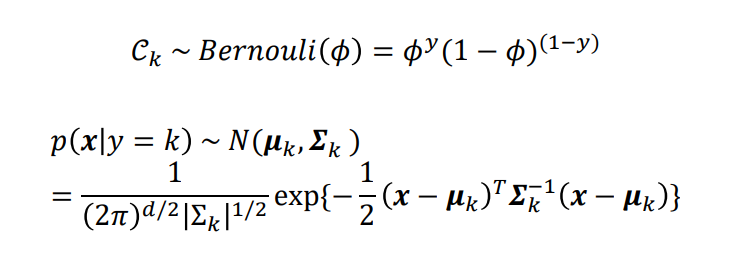
\includegraphics[width=0.35\textwidth]{figs/1.png}
    \label{fig:sample}
\end{figure}

به طور خلاصه امدیم و دامنه را به چند بخش تقسیم کردیم و احتمال وجود در هر قسمت را برابر تعداد سمپل های آن قسمت تقسیم بر تعداد کل سمپل ها قرار دادیم . در اخر برای پیدا کردن $p(x)$ میبینیم که $x$ در کدام قسمت وجود دارد و فرض میکنیم احتمال وجود داشتن در هر بازه به طور یونیفورم در کل بازه تقسیم میشود پس خواهیم داشته که احتمال $x$ برابر است با $p(b_l)$ تقسیم بر طول بازه. 

\subsection{$Non-parametric\:density\:estimation$}
در این قسمت ، از ایده بالا استفاده میکنیم و قسمت های دامنه را انقدر کوچک میکنیم که به معادله حدی برسیم. برای احتمال قرار گرفتن در بازه $R$ خواهیم داشت : 

\[
P = \int_{R} p(x')dx'
\]

حال میخواهیم یک تقریب برای مقدار $P$ ارایه دهیم، میگوییم که احتمال اینکه $k$ نمونه از $n$ نمونه در ناحیه $R$ قرار بگیرند به شکل زیر است : 
\[
P_k = \binom{n}{k} p^k (1-p)^{n-k}
\]

احتمال بالا یک ازمایش برنولی است پس نتیجه میشود که :
\[
E[K] = np 
\]

پس میتوانیم یک تقریب برای $p$ ارایه دهیم : 
\[
p = k / n
\]

حال فرض میکنیم که $p(x)$ تابع ای پیوسته است و قسمت های این توابع آنقدر کوچک هستند که میتوانیم به  $p$ یک عدد ثابت نسبت بدهیم

\begin{align*}
P &= \int_{R} p(x')dx' = p(x) \times V \\
V &= Vol(R) \\
x \in R &\Rightarrow p(x) = \frac{P}{V} \approx \frac{k}{nV}
\end{align}

حال با میل دادن فضای $V$ به صفر، میتوانیم $p(x)$ در ان نقطه را به دست بیاوریم.

برای استفاده از نتیجه بالا ، دو راه داریم. در یک راه $V$ را ثابت میگذاریم و $k$ موبوط به هر قسمت را پیدا میکنیم ، در روش دیگر $k$ را ثابت میگذاریم و $k$ عنصری را پیدا میکنیم که در فضای متغییر $v$ پیدا میشوند.

\subsubsection*{$Parzen\:Windows$}
در این راه ما $V$ هارا مشخص میکنیم که این مقدار برابر $h^d$ است و برای هر سمپل چک میکنیم که ایا این سمپل در این قسمت وجود دارد یا خیر، برای اینکار از $Indicator$ زیر استفاده میکنیم
\[
\phi(u) = 
\begin{cases} 
1 & if  |u_1| \leq \frac{1}{2} \wedge \ldots \wedge |u_d| \leq \frac{1}{2} \\
0 & o.w.
\end{cases}
\]

پس برای تابع احتمال خواهیم داشت : 

\[
p_n(x) = \frac{1}{n} \times \frac{1}{h_n^d} \sum_{i=1}^{n} \phi\left( \frac{x - x^{(i)}}{h_n} \right)
\]
دلیل استفاده از $kernel$  این بود که ما میخواهیم فاصله یک نقطه را از مرکز استفاده کنیم و این فاصله را میتوان به شکل $X^T X$ نشان داد.

مقدار $h$ چه اثری میتواند داشته باشد ؟ 

اگر $h$ خیلی کوچک باشد ، قسمت های دامنه ما کوچک تر خواهند بود پس سمپل های کمتری در انجا قرار میگیرند و این سبب میشود که سمپل های موجود در ان قسمت مهم تر باشند و نویز ها بتوانند اسیب زیادی بزنند 
اما از طرفی اگر $h$ خیلی بزرگ باشد ، تابع احتمال ما بیش از اندازه $smooth$ میشود و به اندازه کافی خوب محیط سمپل را درک نمیکند.

به زبانی دیگر برای تعداد ثابت سمپل $h$  کم باعث واریانس زیاد و $h$ زیاد باعث بایاس زیاد میشود .
قابل به ذکر است که در صورتی که سمپل های نامحدود داشته باشیم ، هرچقدر $h$ بیشتر باشد بهتر است. چون با داشتن $h$ کم تنها مشکل ما واریانس بالا است که این مشکل را سمپل های زیاد ما حل میکنند! (افزایش سمپل باعث کم شدن واریانس میشود )
اما این کار عملی نیست پس برای همین میتوانیم از $cross\:validation$ برای پیدا کردن مقدارمناسب $h$  استفاده کنیم.


باید گفت که این روش برای فضای مسیله با بعد بالا خوب نیست زیرا با بیشتر شدن بعد مسیله ، سمپل های مورد نیاز به طور نمایی افزایش میابد که لزوما به انها دسترسی نداریم.

\subsubsection*{$Kn-Nearest\:Neighbor\:Density\:Estimation$}
در این مدل ، ما $K$ مشخصی تایین میکنیم و $V$ را متغییر قرار میدهیم، و از ابتدای بازه شروع میکنیم و در هنگام رویت کردن $k$ سمپل آن قسمت را  به عنوان $V$ خود جدا میکنیم و به اینکار ادامه میدهیم تا همه سمپل ها رویت شوند.

در این مدل انتخاب $k$ ، $trade\:off$ ای مانند $h$ دارد.  

\subsubsection*{$Complimentary$}
در این مدل ها انتخاب $k$ یا $h$ درست بسیار مهم است.
این مدل ها زمان زیادی برای پردیکشن نیازدارند.
این مدل ها فضای زیادی نیازدارند زیرا تمامی سمپل هارا در خود نگه میدارد.



\subsection{$Instance-based\:learners$}
برای  $classification$ با مدل های بالا کافی است از روشی که برای $generative\:classification$ ها استفاده میکردیم استفاده کنیم. یعنی $prior$ را مانند قبل با استفاده از سمپل ها به دست میاوریم و $posterior$  را با استفاده از تابع احتمال بالا به دست میاوریم و بعد از امتیاز دهی به همه کلاس ها، محتمل ترین کلاس را انتخاب میکنیم.

در ادامه به روش های دیگری میپردازیم که از $Non-parametric\:density\:estimation$ استفاده نمیکنند.

\subsubsection*{$KNN\:classification$}
در این مدل ، برای هر $x$ ، $k$ نزدیک ترین سمپل به $x$ را پیدا میکنیم و کلاسی را به $x$ میدهیم که بیشتر از بقیه کلاس ها در $k$ همسایه  $x$ دیده شده.
قابل ذکر است که استفاده $k$ کوچیک باعث حساس بودن به نویز میشود و استفاده از $k$ بالا ممکن است باعث بایاس بالا شود پس بهتر از با استفاده از $cross\:validation$ یک $k$ مناسب انتخاب کنیم.

\subsubsection*{$Weighted\:(or\:kernel)\:KNN$}
در قسمت قبل ما به همه $k$ عضو همسایه به یک اندازه اهمیت میدادیم ولی این امر باعث از دست رفتن مقداری اطلاعات میشود ، برای مثال میتوان گفت که همسایه های نزدیک تر مهم تر از همسایه های دور تر هستند ، به همین دلیل میتوانیم اثر هر همسایه را وزن دار کنیم و در انتها امتیازهای هر کلاس را برای $x$ در نظر بگیریم و بهترین کلاس را انتخاب کنیم.

این ضریب میتواند برابر با عکس فاصله $x$ با آن همسایه باشد زیرا میخواهیم همسایه های نزدیک تر مهم تر باشند و از انجایی که فاصله را میتوان به شکل $X^TX$ نشان داد ، میتوانیم از کرنل ها برای راحت تر شدن کارمان استفاده کنیم.

در ادامه میتوان اضافه کرد که در حالت قبل ما باید همه سمپل هارا چک کنیم تا $k$ نزدیک ترین همسایه را پیدا کنیم ، پس میتوانیم بجای استفاده نکردن از برخی از سمپل ها ، بدون تغییر در اردر زمانی، از همه سمپل ها استفاده کنیم و دیگر خودمان را به $k$ همسایه محدود نکنیم.

\subsubsection*{$KNN\:regression$}
برای حالت $regression$ ، پروسه ای مانند $classification$ خواهیم داشت با این تفاوت که به جای استفاده از $majority\:vote$ ، $score$ های همسایه هارا میانگین میگیریم . اما این کار میتواند مشکل هایی داشته باشد، 
برای مثال مقدار پیش بینی شده $x$ گسستگی هایی خواهد داشت که میتوانیم با استفاده از وزن ها (برای مثال معکوس فاصله) آنرا را تا حدی رفع کنیم و میتوانیم با استفاده از مقدار $k$ بالاتر این گسستگی هارا $smooth$ تر کنیم که این مقدار $trade\:off$  بایاس واریانسی مانند بخش های قبل دارد.

مانند قسمت $classification$ ، میتوانیم به همسایه ها وزن دهیم و برای بهتر شدن عملکرد به جای بخشی ازسمپل ها از همه سمپل ها استفاده کنیم.

\subsubsection*{$Locally\:linear\:weighted\:regression$}
در این مدل صرفا $k$ همسایه نزدیک $x$ را پیدا میکنیم و با استفاده از این $k$ همسایه ، یک 

$local\:parametric\:regression$ روی این سمپل ها اموزش میدهیم و برای پیش بینی $x$ های آن ناحیه از این $parametric\:regression$ استفاده میکنیم. با اینکار هم از خوبی های $parametric$ و هم از خوبی های $non-parametric$ استفاده کرده ایم.  



\end{document}